\section{An exact test of endpoint cancellation}
\label{sec:global-validation}

We evaluate the full Gaussian $W_2$ formula for
Eq.~\eqref{eq:blind-gaussian-generator} with $a=0.4$,
$\epsilon=0.08$, and compare it with the preserving control
$b(t)=a$.  Both fields generate exactly the same Gaussian path.
The grids are uniform or use
$\rho(t)=1+0.2\cos(2\pi t)$, with $N=16,\ldots,4096$ powers of two.
Every distance below uses the exact scalar covariance recurrence;
there is no empirical optimal-transport estimator or sampling error.

\begin{figure*}[t]
 \centering
 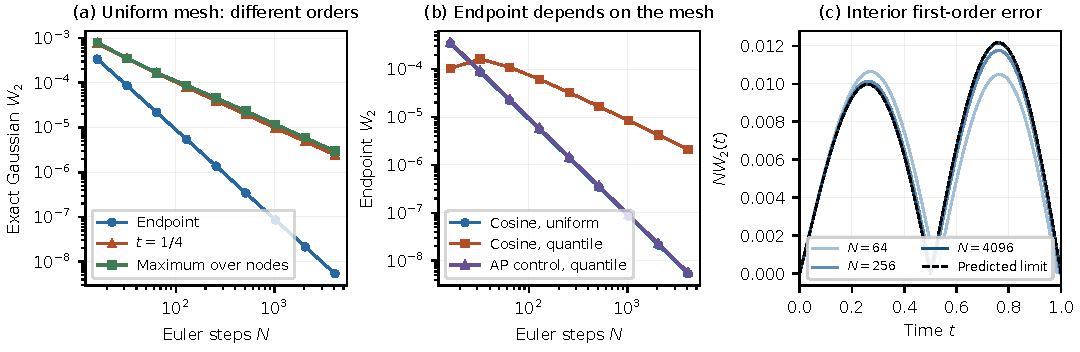
\includegraphics[width=\textwidth]{../results/global_validation/endpoint_cancellation.pdf}
 \caption{Endpoint convergence can conceal a first-order path error.
 The cosine field and the preserving control have the same uniform-grid
 second-order terminal coefficient. The cosine field has first-order
 maximum-node error, and a small allocation perturbation makes its
 terminal error first order as well. Distances are evaluations of exact
 Gaussian formulas.}
 \label{fig:global-validation}
\end{figure*}

\begin{table}[t]
\centering
\caption{Observed orders from $N=2048$ to $4096$.}
\label{tab:global-validation}
\begin{tabular}{llrr}
\toprule
Field & Grid & Terminal & Maximum node\\
\midrule
Cosine & Uniform & 1.9998 & 0.9969\\
Cosine & Perturbed & 0.9955 & 0.9977\\
Preserving & Uniform & 1.9998 & 1.9998\\
Preserving & Perturbed & 1.9998 & 1.9998\\
\bottomrule
\end{tabular}
\end{table}

The analytical terminal coefficient on uniform grids is
$0.0900163721$ for both fields.  For the cosine field,
$N W_2$ at time $1/4$ tends to $0.00995003410$ and the
maximum-node coefficient is $0.0121776345$.  Under the perturbed
allocation, its terminal $N W_2$ tends to $0.00870095137>0$.
At $N=4096$, the cosine field's uniform terminal error is
$5.36463\times10^{-9}$, while its maximum-node error is
$2.96663\times10^{-6}$.  The theorem, rather than a fitted slope,
establishes the orders and limits.

For numerical verification, an independent $2\times2$ covariance
propagation agrees with the scalar recurrence within
$1.05\times10^{-13}$ in absolute covariance. Twelve independent
100-digit reference calculations agree with the stable double-precision
$W_2$ evaluations within $1.45\times10^{-12}$ relative error.
These are arithmetic cross-checks, not interval enclosures.
Eight dedicated tests check the field identity, schedule equation,
independent covariance recurrence, coefficients, and convergence behavior.
The script, CSV files, exact constants, and verification receipts are in
\texttt{results/global\_validation/}; reproduction uses
\texttt{scripts/run\_global\_validation.py}.

This controlled example tests the sharp global theorem and the
finite-validation limitation.  It does not numerically prove the
topological obstruction, whose quantification over all nonlinear fields
requires the analytical argument.
